
%!TEX program = xelatex
\documentclass{ctexbeamer}

\usepackage[bluetheme]{ustcbeamer}

                          %%% ustcbeamer说明 %%%%
%% 宏包使用了TikZ代码形式的背景文件(在子文件夹theme中),默认选项"bluetheme",是科大校徽的蓝色;此外ustcbeamer还内置了红色和黑色主题"redtheme","blacktheme"。

                        %%% 自定义你的主题颜色 %%%
%% 一旦使用了下述命令就会覆盖ustcbeamer的内置颜色选项,你可以设置自己喜欢的RGB色值:
% \definecolor{themecolor}{RGB}{0,150,0} % 这是绿色主题
% \definecolor{themecolor}{RGB}{0,150,150} % 青色主题,也蛮好看的

%% 注意小写rgb和大写RGB表示的色值相差255倍,即RGB{255,255,255}=rgb{1,1,1};
% \definecolor{themecolor}{rgb}{0,0.5,0.3} % 深绿色主题

%% 建议自定义的主题颜色选择偏深色
%%%%%%%%%%%%%%%%%%%%%%%%%%%%%%%%%%%%%%%%%%%%%%%%%%%%%%%%%%%%%%%%%%%%%%


\title[机器学习中的数学基础]{
    机器学习中的数学基础
}
\author[顾言午]{顾言午}
\institute[USTC]{
中国科学技术大学,大数据学院
}
\date{\today}
\begin{document}
%\section<⟨mode specification⟩>[⟨short section name⟩]{⟨section name⟩}
%小于等于六个标题为恰当的标题

%--------------------
%标题页
%--------------------
\maketitleframe
%--------------------
%目录页
%--------------------
%beamer 101
\begin{frame}%
	\frametitle{大纲}%
	\tableofcontents[hideallsubsections]%仅显示节
	%\tableofcontents%显示所节和子节
\end{frame}%
%--------------------
%节目录页
%--------------------
\AtBeginSection[]{
\setbeamertemplate{footline}[footlineoff]%取消页脚
  \begin{frame}%
    \frametitle{大纲}
	%\tableofcontents[currentsection,subsectionstyle=show/hide/hide]%高亮当前节,不显示子节
    \tableofcontents[currentsection,subsectionstyle=show/show/hide]%show,shaded,hide
  \end{frame}
\setbeamertemplate{footline}[footlineon]%添加页脚
}
%--------------------
%子节目录页
%--------------------
\AtBeginSubsection[]{
\setbeamertemplate{footline}[footlineoff]%取消页脚
  \begin{frame}%
    \frametitle{大纲}
	%\tableofcontents[currentsection,subsectionstyle=show/hide/hide]%高亮当前节,不显示子节
    \tableofcontents[currentsection,subsectionstyle=show/shaded/hide]%show,shaded,hide
  \end{frame}
\setbeamertemplate{footline}[footlineon]%添加页脚
}

\section{线性代数}
\subsection{基础概念}
\begin{frame}{基础概念}
    \begin{itemize}
        \item 向量、矩阵与张量
        \item 范数、距离
    \end{itemize}
\end{frame}

\begin{frame}{向量、矩阵与张量}
向量
    \begin{equation*}
        \vec a = \left[
        \begin{array}{cccc}
         0 & 0 & 1 & 1  
    \end{array} \right]^T
    \end{equation*} 
    or
    \begin{equation*}
        \boldsymbol{a} = \left[
        \begin{array}{cccc}
         0 & 0 & 1 & 1  
    \end{array} \right]^T
    \end{equation*} 
矩阵
    \begin{equation*}
        \boldsymbol{A} = \left[
        \begin{array}{cccc}
         1 & x_1 & x_1^2 & x_1^3  \\
         1 & x_2 & x_2^2 & x_2^3  \\
         1 & x_3 & x_3^2 & x_3^3  \\
         1 & x_4 & x_4^2 & x_4^3  \\
    \end{array} \right]
    \end{equation*} 
\end{frame}

\begin{frame}{向量、矩阵与张量}
张量
    \begin{equation*}
        \boldsymbol{A} = \left[
        \begin{array}{cc}
         \left[0,0,0\right] & \left[256,256,0\right]   \\
         \left[0,256,256\right] & \left[256,256,256\right]\\
    \end{array} \right]
    \end{equation*} 
\end{frame}

\begin{frame}{范数、距离}
向量范数:\\
正则化,防止过拟合
    \begin{itemize}
        \item L1范数 $\|x\|_1=\sum_{k=1}^n|x_k|$
        \item L2范数 $\|x\|_2=\sqrt{\sum_{k=1}^nx_k^2}$
        \item 无穷范数 $\|x\|_\infty=\max{|x_k|}$
    \end{itemize}
\end{frame}

\begin{frame}{范数、距离}
矩阵范数:\\
防止过拟合
    \begin{equation*}
        \|A\| = \max\frac{\|Ax\|}{\|x\|}, \|x\|\neq 0
    \end{equation*}
    \begin{itemize}
        \item L1范数 $\|A\|_1=\max_j\sum_{i=1}^m|x_{ij}|$
        \item L2范数 $\|A\|_2=\max \lambda_i(A^HA)$
        \item 无穷范数 $\|A\|_1=\max_i\sum_{j=1}^n|x_{ij}|$
    \end{itemize}
\end{frame}

\begin{frame}{范数、距离}
距离:\\
验证算法效果
    \begin{itemize}
        \item 曼哈顿距离 $d=\sum_{k=1}^n|x_k-y_k|$
        \item 欧氏距离 $d=\sqrt{\sum_{k=1}^n(x_k-y_k)^2}$
        \item 闵可夫斯基距离 $d=\sqrt[p]{\sum_{k=1}^n(x_k-y_k)^p}$
        \item 切比雪夫距离 $d=\max(|x_k-y_k|)$
        \item 夹角余弦 $d=\frac{\sum_{k=1}^nx_ky_k}{\sqrt{\sum_{k=1}^nx_k^2}\sqrt{\sum_{k=1}^ny_k^2}}$
        \item 汉明距离, 两串字符串中不同位数的数目
    \end{itemize}
\end{frame}

\subsection{矩阵的分解算法}
\begin{frame}
  \frametitle{矩阵的分解算法}
  \begin{itemize}
    \item 特征值分解
    \item LU分解
    \item SVD分解
    \item Moore-Penrose伪逆
  \end{itemize}

\end{frame}

\begin{frame}{特征值分解}
    通过旋转变换,将矩阵的主要信息转化到对角线上,主成分分析(PCA)
    \begin{equation*}
        \boldsymbol{A} = \boldsymbol{P}\boldsymbol{\Delta}\boldsymbol{P}^{-1}
    \end{equation*}
    幂方法
\end{frame}

\begin{frame}{LU分解}
    L:下三角矩阵,U:上三角矩阵,便于求矩阵的逆,从而计算
    $$\boldsymbol{Ax=b} $$
    Cholesky分解与Doolitle分解
\end{frame}

\begin{frame}{SVD分解}
    奇异值
    $$\boldsymbol{A}_{m\times n}=\boldsymbol{U}_{m\times m}\boldsymbol{\Sigma}_{m\times n}\boldsymbol{V}_{n\times n}^T$$
    其中
    $$\boldsymbol{U}^T\boldsymbol{U}=\boldsymbol{I},\boldsymbol{V}^T\boldsymbol{V}=\boldsymbol{I}$$
$\boldsymbol{\Sigma}$为对角元为$\sigma_i(A)$的对角矩阵,$\sigma_i(A)=\lambda_i(A^TA)$

QR 分解
\end{frame}

\begin{frame}{Moore-Penrose伪逆}
$$\boldsymbol{A=U\Sigma V^T}$$  
$$\boldsymbol{A^+=V\Sigma^{-1} U^T}$$    
\end{frame}


\section{多元微积分}
\subsection{基本概念}
\subsection{向量函数、方向梯度与海森矩阵}
\begin{frame}{向量函数、方向梯度}
    假设我们有一个以向量为自变量的函数
    $$f(\boldsymbol{x})=f(x_1,x_2,...,x_n)$$
    那么
    \begin{equation*}
    \begin{split}
        df = \frac{\partial f}{\partial x_1}d x_1 + \frac{\partial f}{\partial x_2}dx_2 +...+\frac{\partial f}{\partial x_n}dx_n\\
        =\left(\begin{array}{cccc}
         \frac{\partial f}{\partial x_1}&\frac{\partial f}{\partial x_2}&...&\frac{\partial f}{\partial x_n}
        \end{array}\right)
        \left(\begin{array}{c}
        dx_1\\dx_2\\\vdots\\dx_n
        \end{array}\right)
	\end{split}
            \end{equation*}
    记
    $$\nabla f = \left(\begin{array}{cccc}
         \frac{\partial f}{\partial x_1}&\frac{\partial f}{\partial x_2}&...&\frac{\partial f}{\partial x_n}
        \end{array}\right)$$
\end{frame}



\begin{frame}{海森矩阵}
    记
    $$\nabla^2 f = \left(\begin{array}{cccc}
         \frac{\partial^2 f}{\partial x_1\partial x_1}&\frac{\partial x_1\partial^2 f}{\partial x_2}&...&\frac{\partial^2 f}{\partial x_1\partial x_n}\\
         \frac{\partial^2 f}{\partial x_2\partial x_1}&\frac{\partial^2 f}{\partial x_2\partial x_2}&...&\frac{\partial^2 f}{\partial x_2\partial x_n}\\
         \vdots&\vdots&\ddots\vdots\\
         \frac{\partial^2 f}{\partial x_n\partial x_1}&\frac{ \partial^2 f}{\partial x_n\partial x_2}&...&\frac{\partial^2 f}{\partial x_n\partial x_n}\\
        \end{array}\right)$$
试试对$f(\boldsymbol{x})$进行泰勒展开?
\end{frame}


\subsection{矩阵函数}
\begin{frame}{矩阵函数的一些性质}
\begin{itemize}
    \item $\frac{\partial f(\boldsymbol{A})}{\partial\boldsymbol{A}}= (\frac{\partial f(\boldsymbol{A})}{\partial A_{ij}})_{ij} $
    \item $\frac{\partial \boldsymbol{A}(x)}{\partial x}= (\frac{\partial A_{ij}}{\partial x})_{ij} $
    \item 请注意,求导的链式法则仍然满足
\end{itemize}
我们来推导$\frac{\partial A^{-1}}{\partial x}=-A^{-1}\frac{\partial A}{\partial x}, \frac{\partial \ln det(A)}{\partial A} = A^{-T}$
    
\end{frame}
\begin{frame}{求导的一些公式}
设 $a, \boldsymbol{a,A}$ 均与 $x,\boldsymbol{x}$ 无关,$u,v$ 均有关, $f,u,v$ 可导
\begin{itemize}
    \item $\frac{\partial a\boldsymbol{u}}{\partial x} = a\frac{\partial \boldsymbol{u}}{\partial x}$
    \item $\frac{\partial \boldsymbol{Au}}{\partial x}=\frac{\partial \boldsymbol{u}}{\partial x}\boldsymbol{A}^T$
    \item $\frac{\partial \boldsymbol u^T}{\partial x}=(\frac{\partial \boldsymbol u}{\partial x})^T$
    \item $\frac{\partial f(\boldsymbol u)}{\partial x} = \frac{\partial \boldsymbol u}{\partial x}\frac{\partial f(\boldsymbol u)}{\partial \boldsymbol u}$
    
\end{itemize}
    
\end{frame}

\begin{frame}{求导的一些公式}
设 $a, \boldsymbol{a,A}$ 均与 $x,\boldsymbol{x}$ 无关, $f(\boldsymbol u),\boldsymbol {u(x),v(x)}$ 可导
\begin{itemize}
    \item $\frac{\partial \boldsymbol u^T\boldsymbol v}{\partial \boldsymbol x}=\frac{\partial \boldsymbol u}{\partial \boldsymbol x}\boldsymbol v+\frac{\partial \boldsymbol v}{\partial \boldsymbol x}\boldsymbol u$
    \item $\frac{\partial \boldsymbol{Au}}{\partial \boldsymbol x} = \frac{\partial \boldsymbol u}{\partial \boldsymbol x}A^T$
    \item $\frac{\partial \boldsymbol{x^TA}}{\partial \boldsymbol x} = A$
    \item $\frac{\partial f(\boldsymbol u)}{\partial \boldsymbol x} = \frac{\partial \boldsymbol u}{\partial \boldsymbol  x}\frac{\partial f(\boldsymbol u)}{\partial \boldsymbol u}$
    \item $\frac{\partial \boldsymbol x^T\boldsymbol x}{\partial \boldsymbol x}=2\boldsymbol  x$
    
\end{itemize}
尝试计算 $$\frac{\partial \boldsymbol {u^TAv}}{\partial \boldsymbol x}, \frac{\partial \boldsymbol {axx^Tb}}{\partial \boldsymbol x}$$
    
\end{frame}

\begin{frame}{Draft}

    
\end{frame}


\begin{frame}{求导的一些公式}
设 $a, \boldsymbol{a,A}$ 均与 $x,\boldsymbol{X}$ 无关, $f(\boldsymbol u),\boldsymbol {u(X),v(X)}$ 可导
\begin{itemize}
	\item $\frac{\partial \boldsymbol u^T\boldsymbol v}{\partial \boldsymbol X}=\frac{\partial \boldsymbol u}{\partial \boldsymbol X}\boldsymbol v+\frac{\partial \boldsymbol v}{\partial \boldsymbol X}\boldsymbol u$
    \item $\frac{\partial f(\boldsymbol u)}{\partial \boldsymbol X} = \frac{\partial \boldsymbol u}{\partial \boldsymbol  X}\frac{\partial f(\boldsymbol u)}{\partial \boldsymbol u}$
    \item $\frac{\partial \boldsymbol {a^TXb}}{\partial \boldsymbol X}=\boldsymbol  {ab^T}$
    
\end{itemize}
尝试计算 $$\frac{\partial \boldsymbol {a^TX^TXb}}{\partial \boldsymbol X}$$
    
\end{frame}

\begin{frame}{Draft}

    
\end{frame}

\subsection{一些优化方法}
\subsubsection{凸集和凸函数}
 \begin{frame}{凸集和凸函数}
凸集:给定集合$C\subseteq \mathbb R^n$.若$\forall x,y\in C$满足
$$\forall t \in (0,1), tx + (1 - t)y \in C$$
那么集合$C$为凸集

凸函数:给定一个函数 $f:\mathbb R^n  \mapsto R$.如果满足$dom(f)$是凸集而且 $\forall x, y \subseteq dom(f)$, 
$$\forall t\subset  [0,1],  f(tx + (1-t)y)\leq tf(x)+(1-t)f(y)$$ 
那么函数$f$是凸函数

\end{frame}
 \begin{frame}{判定凸函数}
一阶条件:假设函数$f$可微,那么$f$是凸函数当且仅当 $\forall x,y \in dom(f)$,

$$f(y) \geq f(x)+\nabla f(x)^T (y -x)$$

二阶条件:假设函数$f$二阶可微,那么$f$是凸函数当且仅当 $\forall x \in dom(f)$

$$\nabla^2f(x)\succcurlyeq 0,$$
即海森矩阵半正定

Thm: 假设函数$f$可微凸函数,那么$x$是$f$ 的全局最优当且仅当

$$\nabla f(x) =0$$

\end{frame}

\subsubsection{线性规划问题}
\begin{frame}{线性规划问题}
\begin{equation*}
    \begin{split}
        \min\ \ \ \ \ \ & c^Tx\\
        s.t.\ \ \ \ \ \  & A_ex_e=b_e\\
        & A_ix_i\leq b_i\\
    \end{split}
\end{equation*}
可基于单纯形法或对偶问题求解

\end{frame}

\subsubsection{非线性优化问题}


\begin{frame}{拉格朗日乘子法}
\begin{equation*}
    \begin{split}
        \min\ \ \ \ \ \ & f(x)\\
        s.t.\ \ \ \ \ \  & g(x) = 0\\
    \end{split}
\end{equation*}
转化为考虑 $$\min\ \ f(x)+\lambda g(x)$$,其中$\lambda$ 可以为任意值. 可以直接求导    
\end{frame}

\begin{frame}{非线形优化问题}
\begin{equation*}
    \begin{split}
        \min\ \ \ \ \ \ & c^Tx\\
        s.t.\ \ \ \ \ \  & g_i(x)\geq0, i=1,...,m\\
        & h_i(x)=0, i=1,...,l\\
    \end{split}
\end{equation*}
\end{frame}

\subsubsection{KKT条件}
\begin{frame}{KKT条件}
    \centering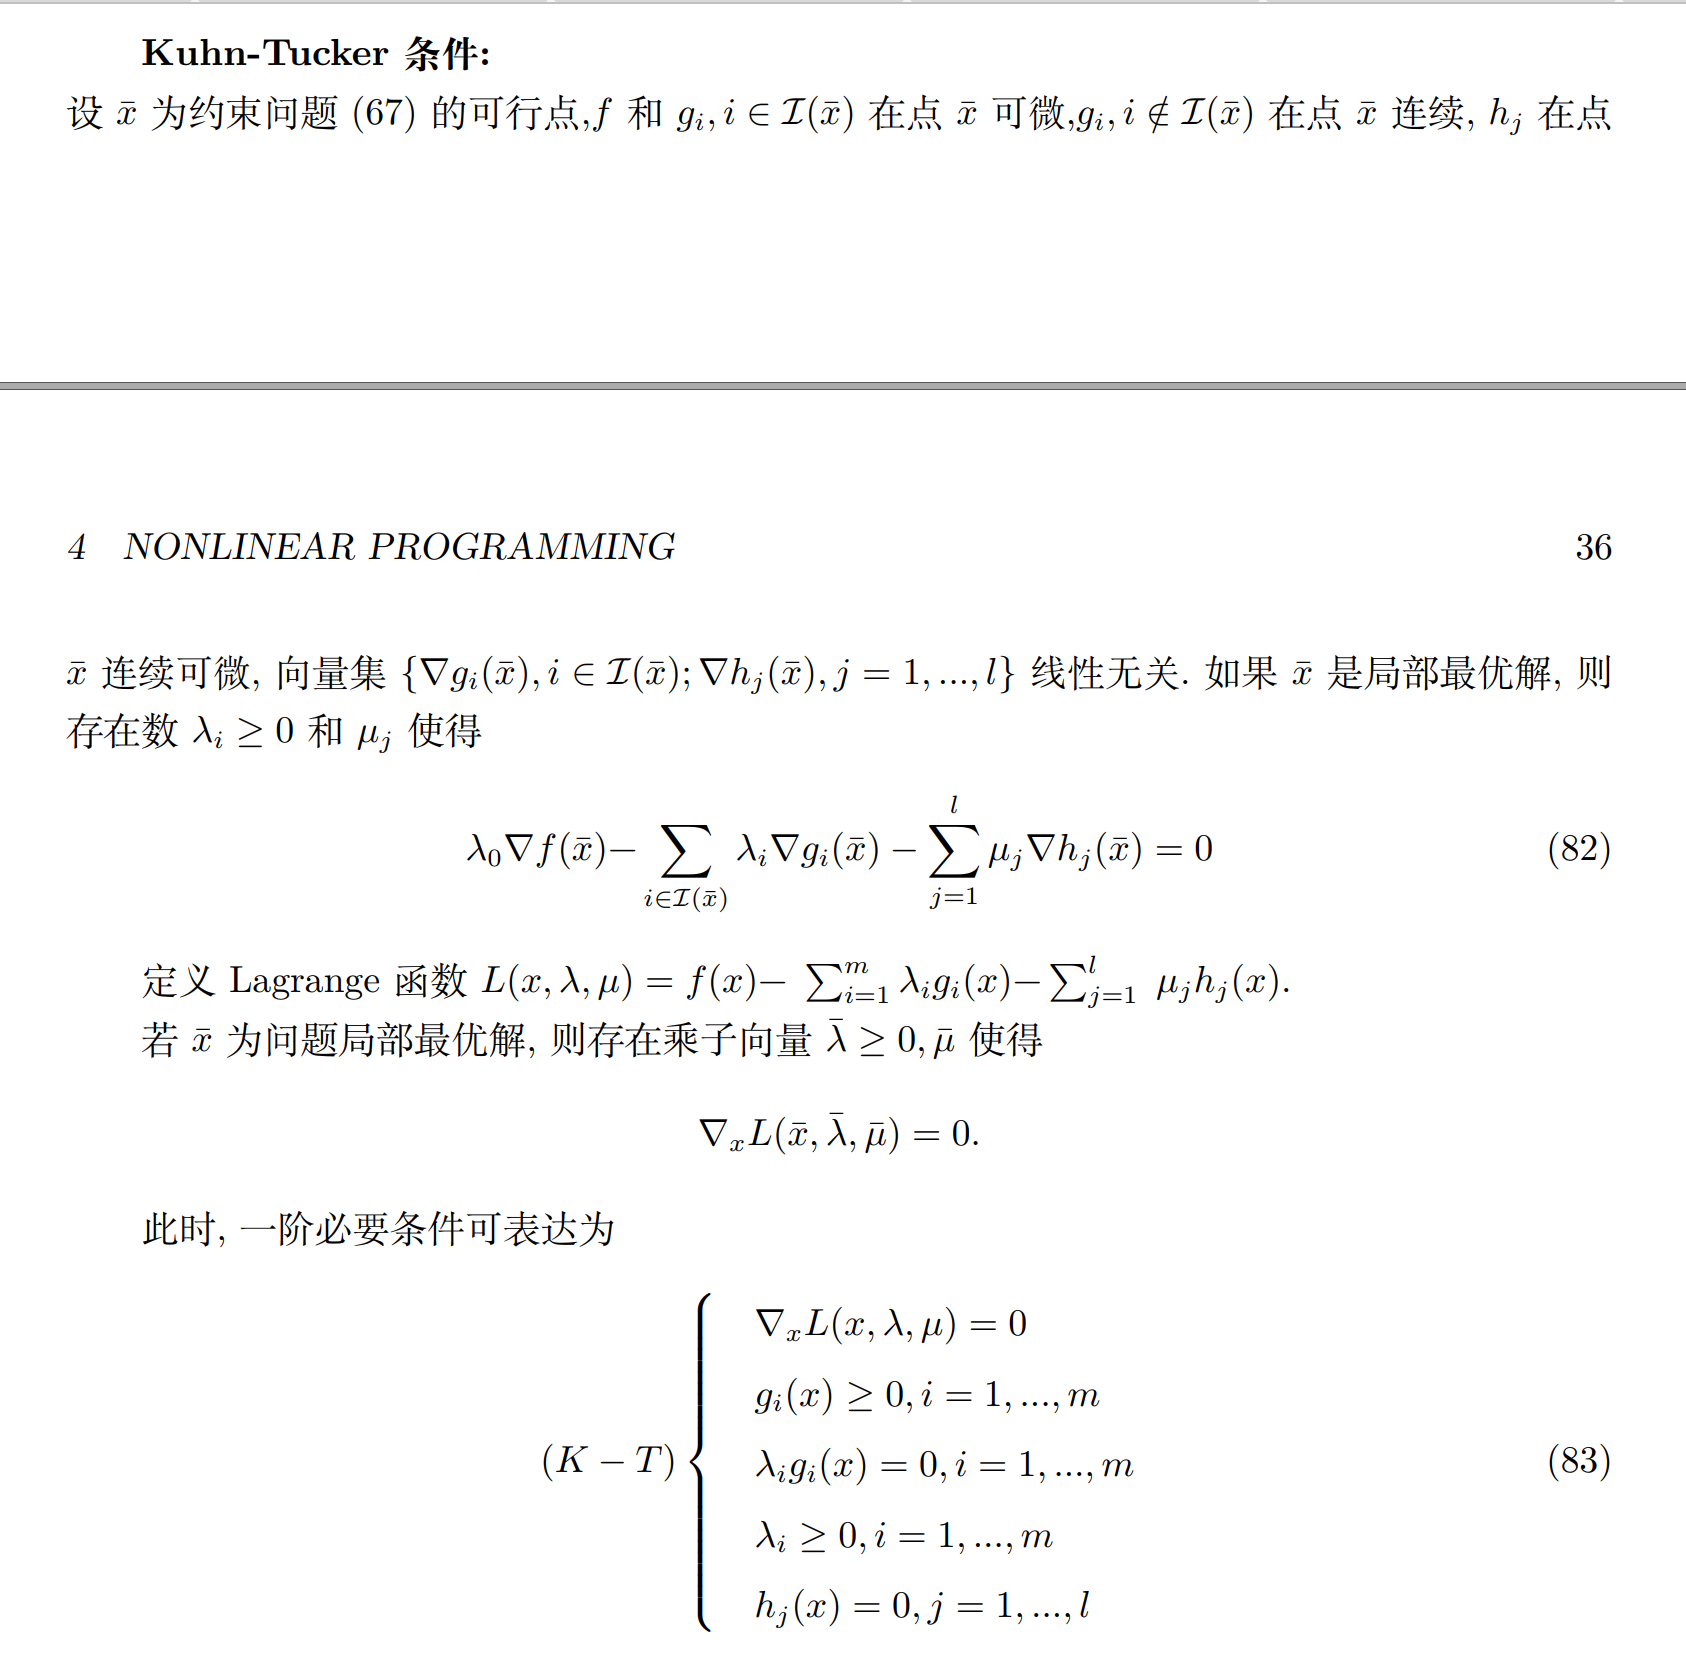
\includegraphics[scale=0.2]{QQ20220902-193038@2x.png}
\end{frame}

\subsubsection{梯度下降法}
\begin{frame}{梯度下降法}
    %$$f(x) = f(x_0) + f'(x_0)(x-x_0) + f''(x_0)(x-x_0)^2$$
    %$$f(\boldsymbol x) = f(\boldsymbol x_0) + \nabla f(\boldsymbol x_0)(\boldsymbol x-\boldsymbol x_0) + \nabla^2 f(\boldsymbol x_0)(\boldsymbol x-\boldsymbol x_0)^2$$
    \begin{equation*}
        \begin{split}
        f(x) &= f(x_0) + f'(x_0)(x-x_0)\\
        0 &= f(x_0) + f'(x_0)(x-x_0)\\
        x &= x_0-\frac{f(x_0)}{f'(x_0)}
        \end{split}
    \end{equation*}
\end{frame}
\begin{frame}{梯度下降法}
    %$$f(x) = f(x_0) + f'(x_0)(x-x_0) + f''(x_0)(x-x_0)^2$$
    %$$f(\boldsymbol x) = f(\boldsymbol x_0) + \nabla f(\boldsymbol x_0)(\boldsymbol x-\boldsymbol x_0) + \nabla^2 f(\boldsymbol x_0)(\boldsymbol x-\boldsymbol x_0)^2$$
    \begin{equation*}
        \begin{split}
        f(\boldsymbol x) &= f(\boldsymbol x_0) + \nabla f(\boldsymbol x_0)(\boldsymbol x-\boldsymbol x_0)\\
        0 &= f(\boldsymbol x_0) + \nabla f(\boldsymbol x_0)(\boldsymbol x-\boldsymbol x_0)\\
        x &= x_0-\frac{f(\boldsymbol x_0)}{\nabla f(\boldsymbol x_0)}
        \end{split}
    \end{equation*}
\end{frame}

\begin{frame}{牛顿法}
$$f(x^{(k)}+s)\approx f(x^{(k)})+g^{(k)T}s+\frac12s^TG_ks$$
$$g^{(k)}=\nabla f(x^{(k)}), G_k=\nabla^2f(x^{(k)})$$
$$\hat s=-G_k^{-1}g^{(k)}$$
\end{frame}





\section{概率论与数理统计}
\subsection{组合、概率规则和公理}
\begin{frame}{组合、概率规则和公理}
请自主复习概率论与数理统计相关知识

大数定律是机器学习的基础
\end{frame}
\subsection{期望与方差}
\begin{frame}{期望与方差}
请自主复习概率论与数理统计相关知识

理解二者不可兼得
\end{frame}
\subsection{分布}
\begin{frame}{分布}
机器学习中比较重要的分布:
\begin{itemize}
\item 0-1分布
\item 几何分布
\item 二项分布
\item (多元)高斯(正态)分布
\item 指数分布
\item 泊松分布
\item 伽玛分布
\item 贝塔分布
\item 迪利克雷分布
\end{itemize}
\end{frame}

\subsection{贝叶斯公式、先验与后验}
\begin{frame}{贝叶斯公式}
$$P(A_i|B)=\frac{P(B|A_i)P(A_i)}{\sum_j P(B|A_j)P(A_j)}$$
or
$$f_{X|Y}(x|y) = \frac{f_{Y|X}(y|x)f_X(x)}{\int_{\mathbb R}f_{Y|X}(y|u)f_X(u)du}$$
\end{frame}
\begin{frame}{先验与后验}
先验:在考虑实验之前,我们首先通过经验给出参数的一个分布

后验:结合先验分布和实验数据,更新我们对先验分布的认知
\end{frame}

\begin{frame}{一个例子}
假设我们的观测值$x$ 服从关于 $\theta$ 的二项分布, $f(x|\theta)=\binom nx \theta^x(1-\theta)^{n-x},x=0,1,...,n$

我们有先验知识,$\theta$服从参数为$\alpha,\beta$的贝塔分布$\pi(\alpha, \beta)=\frac1{B(\alpha,\beta)}\theta^{\alpha-1}(1-\theta)^{\beta-1},0\leq\theta\leq 1$

如果我们观测到了一个值$x$, 那么$y$应该服从什么分布?
\end{frame}
\begin{frame}{一个例子}

\end{frame}

\subsection{最大似然估计和最大后验估计}
\begin{frame}{最大似然估计(MLE)}
极大似然估计的核心思想是:认为当前发生的事件是概率最大的事件。因此就可以给定的数据集,使得该数据集发生的概率最大来求得模型中的参数。
$$L(\theta) = \prod_{i=1}^n P(X_i|\theta), \theta = \arg\max_{\theta} L(\theta)$$

\end{frame}
\begin{frame}{最大后验估计(MAP)}
极大后验估计的核心思想是:允许引入参数的先验分布
$$\theta = \arg\max_{\theta} P(\theta|X) = \arg\max_{\theta} \frac{P(X|\theta)P(\theta)}{P(X)}$$
$$=\arg\max_{\theta} {P(X|\theta)P(\theta)}=\arg\max_{\theta} L(\theta)P(\theta)$$
\end{frame}


\begin{frame}{一个例子}
假设我们对$n$ 个观测点$x_i$ 进行观测得到结果$y_i$,且$y\sim N(w^Tx,\sigma^2)$, 试通过MLE和MAP去计算$\hat w.$
\end{frame}
\begin{frame}{一个例子}

\end{frame}

\begin{frame}{Bayes 估计}
见 https://zhuanlan.zhihu.com/p/86009986
\end{frame}


\section{其他}
\subsection{熵}
\begin{frame}{信息熵}
给出信息熵的公式
$$H(X)=-\sum_{i=1}^np(x_i)log(p(x_i))$$
信息熵H作为对随机实验不确定程度的度量,满足三个规则:
\begin{itemize}
\item $H$是$p$的连续函数;
\item 对于等概结果为$n$的随机实验,$H$是$n$的单调递增函数;
\item 组合可加性
\begin{equation*}
\begin{split}
H_n(p_1,p_2,...,p_n) =& H_{n-1}(p_1+p_2,p_3,...,p_n)\\
&+(p_1+p_2)H_2(\frac{p_1}{p_1+p_2},\frac{p_2}{p_1+p_2})
\end{split}
\end{equation*}

\end{itemize}
\end{frame}
\begin{frame}{交叉熵}
假设现在有一个样本集中两个概率分布$p,q$,其中$p$为真实分布,$q$为非真实分布。假如,按照真实分布$p$来衡量识别一个样本所需要的编码长度的期望即位信息熵$-\sum_{i=1}^np(x_i)log(p(x_i))$. 

如果采用错误的分布$q$来表示来自真实分布$p$的平均编码长度,则应该是交叉熵:
$$H(p,q)=-\sum_{i=1}^np(x_i)log(q(x_i))$$

\end{frame}

\begin{frame}{KL散度}
KL散度公式为:
$$D(p\|q) =  \sum_{i=1}^np(x_i)log(\frac{p(x_i)}{q(x_i)})$$
\begin{itemize}
\item 不对称性
\item 非负性
\end{itemize}

\end{frame}



\begin{frame}
  \frametitle{致谢}
  \centerline{\Large 谢谢!}
\end{frame}

\end{document}

